\documentclass[tikz]{standalone}
\usepackage[T1]{fontenc}
\usepackage[utf8]{inputenc}
\usepackage{pgfplots}
\usepackage{grffile}
\pgfplotsset{compat=newest}
\usetikzlibrary{plotmarks}
\usepgfplotslibrary{patchplots}
\usepackage{amsmath}
\usetikzlibrary{decorations.markings}
\usetikzlibrary{decorations, decorations.text,backgrounds}
\usetikzlibrary{spy}
\usetikzlibrary{shapes.misc}
\usetikzlibrary{external}
\usetikzlibrary{backgrounds}

\tikzset{cross/.style={cross out, draw=black, minimum size=2*(#1-\pgflinewidth), inner sep=0pt, outer sep=0pt},cross/.default={1pt}}

\begin{document}


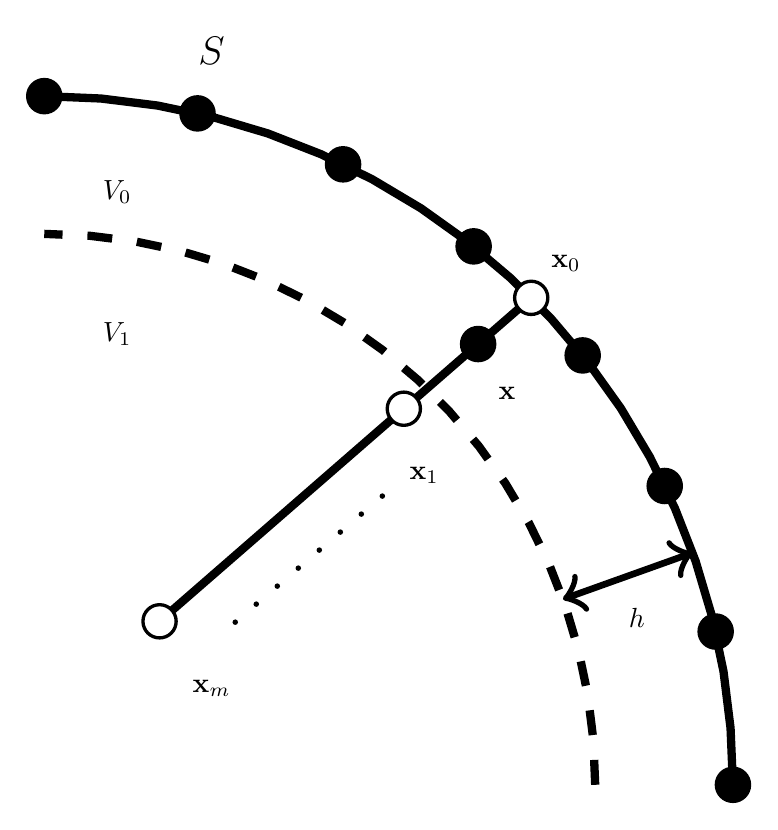
\begin{tikzpicture}[scale=3]

\begin{axis}[
  width=2in, height=2in,
  axis equal,
%  scale only axis,
%  xmin=0, xmax=1.2,
%  ymin=0, ymax=1.2,
  hide axis
  ]
\addplot[color=black,line width =
1.0pt,solid,domain=0:90,samples=20]({cos(\x)},{sin(\x)});
\addplot[color=black,line width =
1.0pt,dashed,domain=0:90,samples=20]({0.8*cos(\x)},{0.8*sin(\x)});
% plot the boundary

\addplot [only marks, mark=*, color=black, fill=black] table{
%1 0
%0.9239 0.3827
%0.7071 0.7071
%0.3827 0.9239
%0 1
1 0
9.7493e-1 2.2252e-1
9.0097e-1 4.3388e-1
7.8183e-1 6.2349e-1
6.2349e-1 7.8183e-1
4.3388e-1 9.0097e-1
2.2252e-1 9.7493e-1
0 1
}; 
% points on the boundary of the geometry 

\addplot [only marks, mark=*,fill=white] coordinates{(0.7071,0.7071)};
\addplot [only marks, mark=*,fill=black] coordinates{(0.6300,0.6400)};
\addplot[color=black,line
width=1.0pt,solid,domain=0:7.2,samples=2]({\x*0.6300+0.7071*(1-\x)},{x*0.6400+0.7071*(1-\x)});
% draw line connecting target point to closest point on boundary
\addplot[only marks, mark=*,fill=white] coordinates {(0.5221,0.5461)};
\addplot[only marks, mark=*,fill=white] coordinates {(0.1674,0.2374)};
% Lagrange interpolation points along 1-d line coming from closest
% point



%\addplot [only marks, mark=*,fill=white] coordinates {(0.6330,0.7742)};
%% open circle which is closest point to curve.  Corresponds to theta =
%% pi/4 + 0.1
%
%%\addplot [color=black,line width = 1.0pt,->,-triangle 60] plot coordinates {(0.6330,0.7742) (1.5*0.6330,1.5*0.7742)};
%% draw the normal vector
%
%\addplot [only marks, mark=*,fill=black] coordinates {(0.5965,0.7004)};
%% plot the target location
%
%
%\addplot[color=black,line
%width=1.0pt,solid,domain=0:10,samples=2]({\x*0.5965+0.6330*(1-\x)},{x*0.7004+0.7742*(1-\x)});
%% draw line connecting target point to closest point on boundary

%\addplot[only marks, mark=*,fill=white] coordinates {(0.2679,0.0369)};
%\addplot[only marks, mark=*,fill=white] coordinates {(0.4869,0.4793)};
% Lagrange interpolation points along 1-d line coming from closest
% point


\addplot [color=black,solid,line width = 0.8pt,<->,name=arrow] plot
coordinates {(0.9415,0.3369) (0.8*0.9415,0.8*0.3369)};
%\addplot [color=black,solid,line width = 0.8pt,->] plot
%coordinates {(0.9808,0.1951) (0.8*0.9808,0.8*0.1951)};
%\addplot [color=black,solid,line width = 0.8pt,<-] plot
%coordinates {(0.9808,0.1951) (0.8*0.9808,0.8*0.1951)};
% width of near zone has an arrow to label its width

\end{axis}

\node[font = \Large] at (1.0,3.4) {$S$};
\node at (2.8,1.0) {$h$};
\node at (2.5,2.5) {$\mathbf{x}_{0}$};
\node at (1.9,1.6) {$\mathbf{x}_{1}$};
\node at (1.0,0.7) {$\mathbf{x}_{m}$};
\node at (2.25,1.95) {$\mathbf{x}$};
\draw[dotted,line cap = round, line width=2pt,dash pattern=on 0pt off
5\pgflinewidth] (1.1,0.98) -- (1.8,1.58);
%\draw[dotted,line cap = round, line width=2pt,dash pattern=on 0pt off
%5\pgflinewidth] (1.1,0.85) -- (1.8,1.45);


%\node at (2.2,2.75) {$\mathbf{x}_{0}$};s
%\node at (2.05,1.55) {$\mathbf{x}_{1}$};
%\node at (1.6,0.3) {$\mathbf{x}_{m}$};
%\node at (1.85,2.35) {$\mathbf{x}$};
%\node[font = \Large] at (0.8,2.85) {$\Omega_{0}$};
%\node[font = \large] at (0.8,2.85) {$\mathtt{Near}(\gamma)$};
%\node[font = \Large] at (0.8,2.0) {$\Omega_{1}$};
%\node[font = \large] at (0.8,2.0) {$\mathtt{Far}(\gamma)$};
%\draw[dotted,line cap = round, line width=2pt,dash pattern=on 0pt off
%5\pgflinewidth] (1.5,0.6) -- (1.9,1.4);

\node at (0.6,2.8) {$V_0$};
\node at (0.6,2.2) {$V_1$};

%\draw[gray,thin] (0,0) grid +(3,4);

\end{tikzpicture}
\end{document}
